\chapter{Teoria dell'informazione}

\begin{figure}[h]
    \centering
    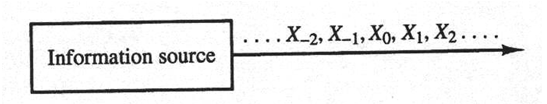
\includegraphics[scale = 1 ]{Sorgente dms.png}
\end{figure}

\newpage 

\section{Modello matematico per una sorgente di informazione}
\footnote{Slide del prof | Teoria dell'informazione | pag 1.1 \\  
Slide | Teoria dell'informazione | pag 1.1 
 }

Le sorgenti di informazione possono essere modellate come processi stocastici, 
le cui proprietà dipendono dalla natura e dalle caratteristiche della sorgente. \newline 

\begin{tcolorbox}
    Ripassati al volo il capitolo sui processi stocastici da Teoria dei segnali perché sarà molto utile. \newline 
    
    Da \url{https://github.com/ciccio25/appunti-teoria-dei-segnali/blob/main/Appunti%20Teoria%20dei%20segnali.pdf} \\
    Capitolo 13 - Processi stocastici - pag 151 - 158
\end{tcolorbox}

Ad esempio questo è lo spettro di un segnale di potenza di una voce umana: 

\begin{figure}[h]
    \centering
    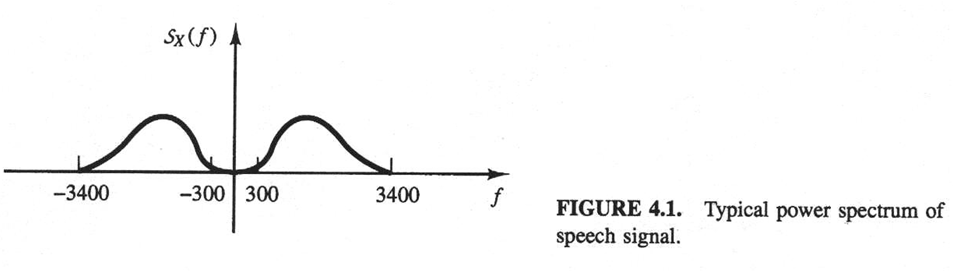
\includegraphics[scale = 0.8]{Spettro di potenza della voce.png}
\end{figure}

\newpage 

\section{Sorgente discreta}
\footnote{Slide del prof | Teoria dell'informazione | pag 1.2 \\
Slide | Teoria dell'informazione | pag 1.2 
}

Consideriamo la seguente sorgente: 

\begin{figure}[h]
    \centering
    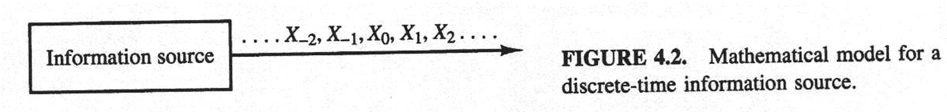
\includegraphics[scale = 0.8]{Sorgente discreta.png}
\end{figure}

cioè una sorgente discreta, cioè che ha un alfabeto di valori finiti e non infiniti, in particolare una sorgente d.m.s., 
cioè una sorgente discreta senza memoria (discrete memoryless sources). \newline 

\begin{tcolorbox}
    d.m.s. non d.r.s. della Formula 1 
\end{tcolorbox}

\newpage 

\subsection{Sorgente d.m.s.}
\footnote{Slide del prof | Teoria dell'informazione | pag 2 \\  
Slide | Teoria dell'informazione | pag 2 
}

In una sorgente d.m.s., i simboli sono generati indipendente a partire da una assegnata (e costante, se la sorgente è stazionario) distribuzione di probabilità. \newline 

Ricordiamo che essendo indipendenti, ogni elemento dell'alfabeto ha covarianza nulla con tutti gli altri elementi. \newline 

La sorgente è caratterizzata da un alfabeto A: 

{
    \Large 
    \begin{equation}
        A = {a_1, a_2, \dots, a_N}
    \end{equation}
}


di valori possibili e una distribuzione di probabilità discrete $p_i$: 

{
    \Large 
    \begin{equation}
        p_i = \Pr{X = a_i} \text{ } \forall i = 1, 2, \dots, N
    \end{equation}
}

Considerando come esempio una sorgente binario, avremo che l'alfabeto A è uguale a: 

{
    \Large
    \begin{equation}
        A = {0, 1}
    \end{equation}
}

Dalla teoria della probabilità, si sa che la probabilità dell'alfabeto è: 

{
    \Large 
    \begin{equation}
        \Pr{A} = 1
    \end{equation}
}

quindi, essendo presenti un due elementi equiprobabili: 

{
    \Large 
    \begin{equation}
        \begin{split}
            \Pr{X = 1} &= \Pr{A} - \Pr{X = 0}
            \\
            &= 1 - \Pr{ X = 0} = p
        \end{split}
    \end{equation}
}

Questa equazione è vera solo se: 

{
    \Large 
    \begin{equation}
        \Pr{X = 1} = \Pr{X = 0}  = p = 0.5
    \end{equation}
}

Quando $p= 0.5$, si dice che è una sorgente binaria simmetrica (o b.s.s.), che è un caso particolare. \newline 

\newpage 

\section{Misura dell'informazione}
\footnote{Slide del prof | Teoria dell'informazione | pag 3.1 \\  
Slide | Teoria dell'informazione | pag 3.1 
}

Prima di parlare e discutere di informazione, dobbiamo specificare cosa si intende per informazione. \newline 

\begin{tcolorbox}
    
\includegraphics[scale = 0.5]{giuseppe-conte-nomi-e-cognomi.jpg}
\end{tcolorbox}

Per informazione si intende la riduzione di incertezza che si può calcolare a priori sul verificarsi di un evento. \newline 

L'informazione associata ad un evento dipende dalla probabilità dell'evento: più la probabilità è bassa, più l'informazione è elevata. \newline 

\begin{tcolorbox}
    Immagina di conoscere una coppia che è fidanzata da anni. \newline
    
    Per te è più una informazione che ieri si sono lasciati o che ieri hanno comprato il gelato? \newline 

    Ovviamente, l'informazione è che si sono lasciati (se sei uno come me, sarebbe più interessato al gelato perché vorrebbe sapere se il gelato è buono e dove lo hanno comprato, ma questo è un altro discorso) 
    perché, prima di oggi, sapevi che stavano bene insieme e non avevano mai litigato. 

\end{tcolorbox}

Un evento certo non "porta" informazione. \newline 

\begin{tcolorbox}
    Se io accendo il fornello, 
    è una informazione farsi male toccando il fuoco con la mano? \newline 
    
    No, non lo è (a meno che non sei masochista, ma qui, come scritto prima, non consideriamo i casi particolari), 
    perché sicuramente ti farai male. \newline 
    
    Quindi toccare con una mano il fuoco non è una informazione perché è certa. 
\end{tcolorbox}

L'informazione non cambia in modo significativo se la probabilità non varia in modo significativo. \newline 

\begin{tcolorbox}
    Se sai che domani pioverà e piuttosto che piovere per 30 minuti, l'app del meteo ti mando una notifica in cui ti informa che domani pioverà per 35 minuti. \newline 

    La notifica dell'app del meteo è informativa? \newline 

    Si, lo è, ma 35 minuti di pioggia non sono tanto diversi dai 30 minuti che sapevi prima della notifica.
\end{tcolorbox}

Una proprietà molto importante di due eventi indipendenti, e che quindi hanno covarianza nulla, 
l'informazione ad essi associata è uguale alla somma delle informazioni degli eventi singoli. \newline 

\begin{tcolorbox}
    Prima di andare avanti, ripassati al volo la teoria assiomatica di Kolmogorov, 
    che è la base della teoria della probabilità. \newline 

    \url{https://github.com/ciccio25/appunti-teoria-dei-segnali/blob/main/Appunti%20Teoria%20dei%20segnali.pdf} \\
    Capitolo 12.2 - Teoria assiomatica di Kolmogorov - pag 114 - 115 \newline 

    In particolare, uno dei punti della Teoria assiomatica di Kolmogorov è la seguente. \newline 

    Dati due eventi A e e B mutuamente esclusivi 
    (ovvero incompatibili, cioè tali che non possano verificarsi contemporaneamente) la probabilità dell'evento unione è data dalla somma delle probabilità dei singoli eventi, si ha cioè: 
    {
        \Large 
        \begin{equation}
            A \cup B = \emptyset 
            \rightarrow 
            \Pr{A \cup B} = \Pr{A} + \Pr{B}
        \end{equation}
    }
\end{tcolorbox}

\newpage 

\section{Auto-informazione}
\footnote{Slide del prof | Teoria dell'informazione | pag 3.2 \\  
Slide | Teoria dell'informazione | pag 3.2 \\
Appunti | 2025-07-08 Ricevimento | pag 1.2 }

Dato un evento (ad esempio la generazione di un simbolo $a_j$ da parte di una sorgente) con probabilità $p_j$, 
l'auto-informazione viene indicata con $I(p_j)$. \newline 

L'auto-informazione gode delle seguenti proprietà: 

\begin{itemize}
    \item è una funzione continua di di $p_j$ 
    \item è una funzione decrescente del suo argomento 
    \item se $p_j = p_{j1} \cdot p_{j2}$ allora $I (p_j) = I (p_{j1}) + I (p_{j2})$
\end{itemize}

Si può dimostrare che l'unica funzione in grado di soddisfare queste proprietà è la funzione logaritmo. \newline 

In particolare, da una probabilità $p_j$, possiamo esprimere la sua auto-informazione come: 

{
    \Large 
    \begin{equation}
        I (p_j) = - \log(p_j)
    \end{equation}
}

La base del logaritmo non è importante, ma definisce l'unità con cui si esprime l'informazione. \newline 

Se la base del logaritmo è 2, l'informazione è espressa in bit. \newline 

Se la base del logaritmo è in base e, cioè $\ln$, l'informazione è espressa in nat. \newline 

\begin{tcolorbox}
    Siccome abbiamo a che fare con sistemi digitali, abbiamo a che fare sempre con: 

    {
        \Large 
        \begin{equation}
            I (p_j) = - \log_2(p_j)
        \end{equation}
    }

    Nelle slide sarà solo indicato log. \newline 

    La proprietà dell'auto-informazione che esprime che "una funzione decrescente del suo argomento" si intende l'argomento del logaritmo. \newline 

    Sapendo che l'informazione di $p_j$ possiamo scriverla come, applicando le proprietà del logaritmo: 

    {
        \Large 
        \begin{equation}
            \begin{split}
              I (p_j) &= - \log_2(p_j)
              \\
              &\quad
              \\
              &= \log_2 (p_j)^{-1}
              \\
              &\quad
              \\
              &= \log_2 \left(\frac{1}{p_j} \right)
            \end{split}
        \end{equation}
    }
    
    All'aumentare di $p_j$, l'argomento del logaritmo diminuisce e tende a zero per $p_j$ che tende ad infinito. 
\end{tcolorbox}


\newpage 

\subsection{Contenuto informativo di una d.m.s.}
\footnote{Slide del prof | Teoria dell'informazione | pag 4.1 \\  
Appunti di Damiano| pag 4.1 \\
Slide | Teoria dell'informazione | pag 4.1} 

Consideriamo una d.m.s. (discrete memoryless source): 

\begin{figure}[h]
    \centering
    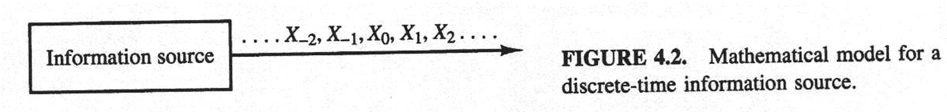
\includegraphics[scale = 0.8]{Sorgente discreta.png}
\end{figure}

Consideriamo la media "pesata" delle auto-informazioni dei simboli della sorgente. \newline 

{
    \Large 
    \begin{equation}
        \sum_{i = 1}^{N}
        p_i \cdot I(p_i)
    \end{equation}
}


La media-pesata delle auto-informazioni prende il nome di entropia, in questo caso la entropia della sorgente. \newline 

Andando a segnare con H(X) l'entropia della sorgente d.m.s. come: 

{
    \Large 
    \begin{equation}
        \begin{split}
        H(X)
        &= 
        \sum_{i = 1}^{N}
        p_i \cdot I(p_i)
        \\
        &=
        \sum_{i = 1}^{N}
        p_i \cdot \left[ - \log_{2} (p_i)\right]
        \\
        &=
        -
        \sum_{i = 1}^{N}
        p_i \cdot \log_{2} (p_i)
        \\
        &= 
        \sum_{i = 1}^{N}
        p_i \cdot  \log_{2} \left(\frac{1}{p_i} \right)
        \end{split}
    \end{equation}
}

\newpage 

\subsubsection{Entropia binaria}
\footnote{Slide del prof | Teoria dell'informazione | pag 4.2 \\  
Appunti di Damiano| pag 4.2 \\
Slide | Teoria dell'informazione | pag 4.2 }

Per una sorgente d.m.s. binaria, abbiamo che l'entropia H(X) è uguale a: 

{
    \Large
    \begin{equation}
        \begin{split}
            H(X)
            &=
            \sum_{i = 1}^{N}
            p_i \cdot I(p_i)
            \\
            &=
            -
            \sum_{i = 1}^{2}
            p_i \cdot \log_{2}(p)
            \\
            &= 
            - p \cdot \log_{2} (p)
            - (1 - p) \cdot \log_{2} (1 - p)
        \end{split}
    \end{equation}
}

Posiamo visualizzare H(X) in questa maniera: 

\begin{figure}[h]
    \centering
    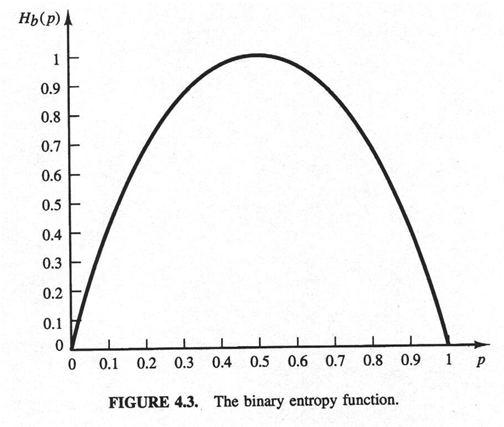
\includegraphics[scale = 1]{entropia dms per una sorgente binaria.png}
\end{figure}

H(X) è una funzione che ha le seguenti caratteristiche: 

\begin{itemize}
    \item concava 
    \item simmetrica 
    \item ha un massimo per $p = \frac{1}{2}$
\end{itemize}

Se 0 e 1 sono equiprobabili, la sequenza binaria è una sequenza di bit (informativi). \newline 

Se p si discosta da $\frac{1}{2}$, alcuni elementi binari non portano informazioni, quindi non tutti gli 0 e 1 sono bit (informativi). \newline 

\begin{tcolorbox}
Per bit si intendono solo quelli che portano una informazione e questa è la definizione nella teoria dell'informazione. \newline 

Nella realtà, il termine bit viene spesso usato come sinonimo di 0 e 1. 
\end{tcolorbox}

\newpage 

\subsubsection{Entropia massima}
\footnote{Slide del prof | Teoria dell'informazione | pag 5 \\  
Appunti di Damiano| pag 5 \\
Slide | Teoria dell'informazione | pag 5 \\
Appunti | 2025-07-08 Ricevimento | pag 1.1}

Graficamente una funzione di distribuzione discreta uniforme, ha il seguente andamento: 

\begin{figure}[h]
    \centering
    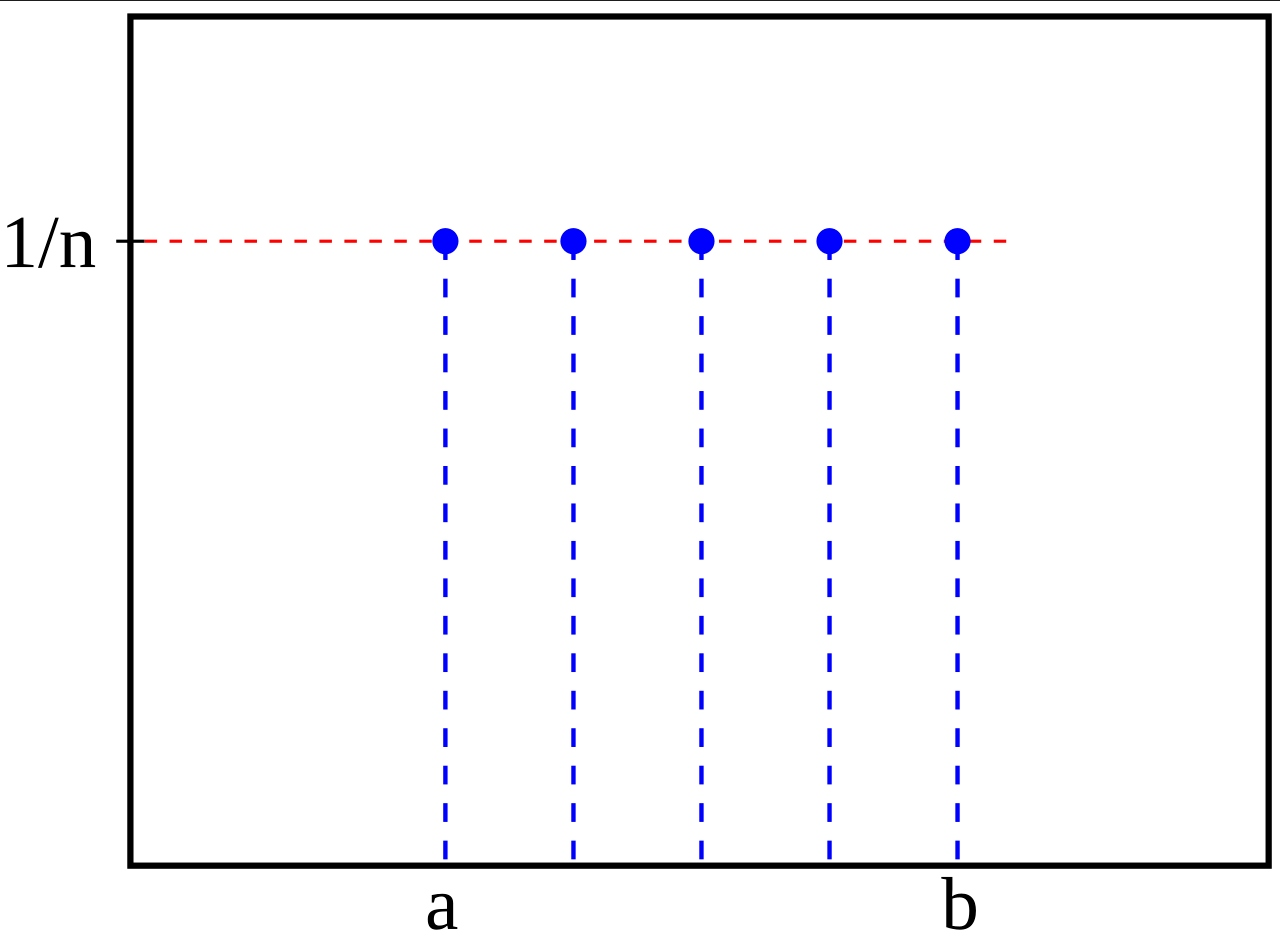
\includegraphics[scale = 0.15]{1280px-DUniform_distribution.svg.jpg}
\end{figure} 

dove N è il numero degli elementi dell'alfabeto A. \newline 

Questo perché, data la formula di H(X), sappiamo che: 

{
    \Large 
    \begin{equation}
        \begin{split}
            H(X) &= 
            \sum_{i = 1}^{N} 
            p_i \cdot I(p_i)
            \\
            &= 
            \sum_{i = 1}^{N}
            p_i \cdot \log_{2} \left(\frac{1}{p_i} \right) 
        \end{split}
    \end{equation}
}

Sapendo che per una funzione di distribuzione discreta uniforme, la probabilità di ogni singolo N elemento dell'alfabeto i $p_i$ vale: 

{
    \Large 
    \begin{equation}
        p_i = N
    \end{equation}
} 

allora: 

{
    \Large 
    \begin{equation}
        \begin{split}
        H (X)
        &= 
        \sum_{i = 1}^{N}
        p_i \cdot \log_{2} \left(\frac{1}{p_i} \right) 
        \\
        &= 
        -
        \sum_{i = 1}^{N}
        p_i \cdot \log_{2} \left(p_i \right) 
        \\
        &\downarrow
        \\
        H(X)
        &=
        -  
        \sum_{i = 1}^{N}
        \frac{1}{N} \cdot \log_{2} \left( N \right)
        \\
        &= 
        -
        \sum_{i = 1}^{N}
        \frac{1}{N} \cdot \log_{2} \left( N\right)
        \\
        &=
        - 
        \log_{2} \left( N\right)
        \cdot 
        \sum_{i = 1}^{N}
        \frac{1}{N}
        \\
        &=
        -
        \log_{2} \left( N\right)
        \cdot 
        1 
        \\
        &=
        - 
        \log_{2} \left( N\right)
        \end{split} 
    \end{equation}
}

Dal secondo al terzo passaggio (contando come prima la sostituzione con $p_i = \frac{1}{N}$), 
posso portare fuori dalla sommatoria il termine $\log_{2} \left( N\right)$ perché è comune a tutti i termini della sommatoria stessa. \newline 

Dal terzo al quarto passaggio, $\sum_{i = 1}^{N} \frac{1}{N} = 1$ per definizione di funzione di distribuzione discreta (la probabilità di tutti gli elementi di un alfabeto è del 100 \% quindi 1). \newline 

Per una sorgente d.m.s., si avrà entropia massima se si ha una funzione di distribuzione discreta uniforme: di seguito la dimostrazione. \newline 

Consideriamo H(X) una entropia generica e $H_{max} (X)$ l'entropia di una funzione di distribuzione discreta uniforme. \newline 

Possiamo scrivere che: 

{
    \Large 
    \begin{equation}
        \begin{split}
            H(X) + H_{max} (X) 
            &=
            -
            \sum_{i = 1}^{N} p_i \cdot \log_{2} \left( p_i \right)
            - \log_{2} (N)
            \\
            &= 
            \sum_{i = 1}^{N} p_i \cdot \log_{2} \left( \frac{1}{p_i} \right)
            +
            \log_{2} \left(\frac{1}{N} \right)
            \\
            &= 
            \sum_{i = 1}^{N} p_i \cdot \log_{2} \left( \frac{1}{p_i \cdot N} \right)
        \end{split} 
    \end{equation}
}

Siccome vogliamo trovare un massimo, questa sommatoria è minore uguale a: 

{
    \Large 
    \begin{equation}
        \begin{split}
            \sum_{i = 1}^{N} p_i \cdot \left( \frac{1}{p_i \cdot N} - 1\right) \cdot \log_{2} \left( e \right)
            &= 
            \left( \sum_{i = 1}^{N} \frac{1}{N} - \sum_{i = 1}^{N} p_i\right) \cdot \log_{2} \left( e \right)
            \\
            &= 
            \left( \sum_{i = 1}^{N} \frac{1}{N} - \sum_{i = 1}^{N} \frac{1}{N}\right) \cdot \log_{2} \left( e \right) 
            \\
            &= 
            (1- 1) \cdot \log_{2} \left( e \right)
            \\
            &= 
            0 \cdot \log_{2} \left( e \right)
            \\
            &= 
            0
        \end{split}
    \end{equation}
}

Mettendo insieme le due equazione abbiamo che: 

{
    \Large 
    \begin{equation}
        \begin{split}
            H(X) + H_{max} (X) &\le 0 
            \\
            &\downarrow
            \\
            H(X)  &\le - H_{max} (X)
            \\
            & \le - \left[ - \log_{2} (N)\right]
            \\
            & \le \log_{2} (N)
        \end{split}
    \end{equation}
}

Quindi, alla fine della dimostrazione abbiamo che, data qualsiasi entropia H(X) essa è sempre minore o uguale all'entropia massima, che vale $\log_{2} (N)$. \newline 

In formule:

{
    \Large 
    \begin{equation}
        H (X) \le \log_{2} (N)
    \end{equation}
}

dove N sono gli elementi dell'alfabeto. \newline 

\begin{tcolorbox}
    Un altro metodo per capire e visualizzare meglio cosa si intende per entropia, ti lascio questo video di TED-ed. \newline 

    \url{https://www.youtube.com/watch?v=YM-uykVfq_E}\\
    Cos'è l'entropia? | Jeff Phillips by TED-ed \newline 

    Nel caso nostro dell'entropia collegata alla probabilità, in particolare all'entropia massima, è meglio questo video: \\

    \url{https://youtu.be/2s3aJfRr9gE?si=J37vVjWY5SWied3H}\\ 
    Information entropy | Journey into information theory | Computer Science | Khan Academy by Khan Academy Labs \newline 

    Se vuoi andare più a fondo, c'è il mitico Josh Starmer (mitico perché l'ho scoperto quando stavo facendo un progetto sulle reti neurali ed io non sapevo nulla sull'argomento, persona molto coinvolgente): \newline 

    \url{https://youtu.be/YtebGVx-Fxw?si=9O2P-pN-lX6nAi3j} \\
    Entropy (for data science) Clearly Explained!!! by StatQuest with Josh Starmer \newline 

    Una nota riguardo alle funzioni di probabilità e la differenza tra le materie. \newline

    Nella probabilità, dobbiamo considerare l'opposto rispetto al corso di misure. Se PDF uniforme è il caso peggiore in misure, qui è il caso migliore. \newline 
    
    Se PDF gaussiano è il caso migliore nelle misure, qui è il caso peggiore perchè ci saranno dei valori più probabili rispetto agli altri dell'alfabeto.  
\end{tcolorbox}

\newpage 

\subsubsection{Entropia congiunta}
\footnote{Slide del prof | Teoria dell'informazione | pag 6.1 \\  
Appunti di Damiano| pag 6.1 \\
Slide | Teoria dell'informazione | pag 6.1 \\
Appunti | 2025-03-21 | pag 2
 }

\begin{tcolorbox}
    Se vuoi "divertirti" a capire meglio l'entropia congiunta, ti consiglio questo video: \newline 

    \url{https://youtu.be/6ArSys5qHAU?si=0KeUXNtcMn2lytFE} \\
    Neural Networks Part 6: Cross Entropy by StatQuest with Josh Starmer

\end{tcolorbox}

L'entropia, come descritto precedentemente, descrive un comportamento medio del sistema. \newline 

Dall'entropia per una variabile X, possiamo esprimere l'entropia per due variabili (X, Y) come: 

{
    \Large 
    \begin{equation}
        H (X, Y)
        = 
        - \sum_{x ,y}
        p(x, y) \cdot \log_{2} \left[ p(x,y)\right]
    \end{equation}
}

dove: 

\begin{itemize}
    \item $\sum_{x ,y}$ si intende la somma di tutti i valori dell'alfabeto X e la somma di tutti valori dell'alfabeto Y 
    \item $ p(x, y)$ è la probabilità congiunta tra l'elemento x e y
\end{itemize}


\begin{tcolorbox}
    \url{https://github.com/ciccio25/appunti-teoria-dei-segnali/blob/main/Appunti%20Teoria%20dei%20segnali.pdf} \\
    Capitolo 12.2 Teoria assiomatica di Kolmogorov - pag 114 - 115 \newline 

    Dati due eventi A e B, la probabilità dell'evento unione $A \cup B$ è espressa dall'uguaglianza:
    {
        \Large 
        \begin{equation}
            \Pr{A \cup B} = \Pr{A} + \Pr{B} + \Pr{A \cap B}
        \end{equation}
    } 

Data una coppia di eventi A e B, la probabilità dell'evento intersezione, spesso indicata semplicemente con $\Pr{A, B}$, è detta probabilità congiunta, 
mentre $\Pr{A}$ e $\Pr{B}$ hanno il significato di probabilità marginali. \newline 

$\blacksquare$ \newline 

Ma per eventi indipendenti, la definizione cambia. \newline 

 \url{https://github.com/ciccio25/appunti-teoria-dei-segnali/blob/main/Appunti%20Teoria%20dei%20segnali.pdf} \\
    Capitolo 12.5 Eventi statisticamente indipendenti - pag 118 - 119 \newline 

    Per eventi indipendenti: 

{   
    \Large 
    \begin{equation}
        \Pr{A, B} = \Pr{A} \cdot \Pr{B}   
    \end{equation}
}

e cioè, che la probabilità congiunta è uguale al prodotto delle probabilità marginali (dei singoli eventi). \newline 

\end{tcolorbox}

Considerando il caso più generale con n variabili \textbf{X}: 

{
    \Large 
    \begin{equation}
        \textbf{X} = (X_1, X_2, \dots, X_n)
    \end{equation}
}

si può estendere la definizione di entropia alle n variabili come: 

{
    \Large 
    \begin{equation}
        H (\textbf{X}) 
        = 
        - 
        \sum_{x_1, x_2, \dots, x_n}
         p(x_1, x_2, \dots, x_n) \cdot \log_{2} \left[ p(x_1, x_2, \dots, x_n)\right]
    \end{equation}
}

\newpage 

\subsubsection{Entropia condizionata}
\footnote{Slide del prof | Teoria dell'informazione | pag 6.2 \\  
Appunti di Damiano| pag 6.2 \\
Slide | Teoria dell'informazione | pag 6.2 \\
Appunti | 2025-03-21 | pag 2
 }

\begin{tcolorbox}
    Beccatevi il socio Josh Starmer. \newline 

    \url{https://youtu.be/eJIp_mgVLwE?si=lJD4NI1HlypPZRro} \\
    Mutual Information, Clearly Explained!!! by StatQuest with Josh Starmer \newline 

    "Mutual Information" proprio perchè, come abbiamo scritto precedentemente, per noi, nella teoria dell'informazione, 
    maggiore entropia significa maggiore informazione. \newline 

    Più casino c'è, più informazione c'è. 
\end{tcolorbox}


Come nella probabilità, anche nell'entropia possiamo considerare l'entropia condizionata. \newline 

Se consideriamo solo un elemento nell'alfabeto y, cioè $Y = y$, 
allora possiamo formulare l'entropia condizionata tra X e Y come: 

{
    \Large 
    \begin{equation}
        X (X | Y = y)
        = 
        - 
        \sum_{x}
        p(x | y) \cdot \log_{2} \left[ p(x | y) \right]
    \end{equation}
}

Invece, considerando tutti i possibili valori di Y, e non uno singolo come prima, 
possiamo scrivere, facendo alcuni passi algebrici:

{
    \Large 
    \begin{equation}
        \begin{split}
            H (X | Y)
            &= 
            -
            \sum_{x}
            \sum_{y}
            p(y) \cdot p (x | y) \cdot \log_{2} \left[ p (x | y )\right] 
            \\
            &= 
            \sum_{x, y} 
            p(x, y) \cdot \log_{2} \left[ p(x | y)\right]
        \end{split}
    \end{equation}
}

dove $p(x | y)$ prende il nome di probabilità condizionata di x su y. \newline 

\begin{tcolorbox}

    \url{https://github.com/ciccio25/appunti-teoria-dei-segnali/blob/main/Appunti%20Teoria%20dei%20segnali.pdf} \\
    Capitolo 12.2 Teoria assiomatica di Kolmogorov - pag 114 - 115 \newline 

    Data una coppia di eventi A e B con $\Pr{B} \neq 0$, si definisce poi la probabilità condizionata: 

{
    \Large 
    \begin{equation}
        \begin{split}
            \Pr{A | B} 
            &= 
            \frac{\Pr{A \cup B}}{\Pr{B}} 
            \\
            &= 
            \frac{\Pr{A, B}}{\Pr{B}}     
        \end{split}
    \end{equation}
} 

la quale esprime la probabilità dell'evento A condizionata al verificarsi dell'evento B (che ha dunque il significato di evento condizionante). \newline 

$\blacksquare$ \newline

Per eventi statisticamente indipendenti invece, dobbiamo utilizzare la formula di Bayes. \newline 

 \url{https://github.com/ciccio25/appunti-teoria-dei-segnali/blob/main/Appunti%20Teoria%20dei%20segnali.pdf} \\
    Capitolo 12.5 Eventi statisticamente indipendenti - pag 118 - 119 \newline 

    Un altro importante risultato è il teorema (o formula) di Bayes, che può essere formalizzato nel modo seguente: 

{
    \Large 
    \begin{equation}
        \Pr{A | B} = \frac{\Pr{B | A} \cdot \Pr{A}}{\Pr{B}}
    \end{equation}
} 

La formula di Bayes è spesso usata in combinazione con il teorema della probabilità totale. \newline 

\end{tcolorbox}

Possiamo generalizzare l'entropia condizionata per n variabili: 

{
    \Large 
    \begin{equation}
        H (X_n | X_1, X_2, \dots, X_{n-1}) 
        = 
        - 
        \sum_{x_1, x_2, \dots, x_n}
         p(x_1, x_2, \dots, x_n) \cdot \log_{2} \left[ p(x_1 | x_2, \dots, x_n)\right]
    \end{equation}
}

\newpage 

\subsection{Legame tra entropia condizionata ed entropia congiunta}
\footnote{Slide del prof | Teoria dell'informazione | pag 7.1 \\  
Appunti di Damiano| pag 7.1 \\
Slide | Teoria dell'informazione | pag 7.1 \\
Appunti | 2025-03-21 | pag 2
}

Di seguito la dimostrazione del legame tra una entropia condizionata $H (X | Y)$ 
ed entropia congiunta $H(X , Y)$: 

{
    \Large 
    \begin{equation}
        \begin{split}
            H(X, Y)
            &= 
            - \sum_{x, y} 
            p(x , y)
            \cdot 
            \log_{2}
            \left[
                p(x, y)
            \right]
            \\
            &= 
            - \sum_{x, y} 
            p(x , y)
            \cdot 
            \log_{2}
            \left[
                p(y)
                \cdot 
                p(x | y)
            \right]
            \\
            &=
            - \sum_{x, y} 
            p(x , y)
            \cdot 
            \log_{2}
            \left[
                p(y)
            \right]
            \\
            &=
            - \sum_{x, y} 
            p(x , y)
            \cdot 
            \log_{2}
            \left[
                p(x | y)
            \right]
            \\
            &=
            - \sum_{x, y} 
            p(y)
            \cdot 
            \log_{2}
            \left[
                p(y)
            \right]
            \\
            &=
            - \sum_{x, y} 
            p(x, y)
            \cdot 
            \log_{2}
            \left[
                p(x | y)
            \right]
            \\
            &= 
            H(Y) + H(X | Y)
        \end{split}
    \end{equation}
}

cioè: 

{
    \Large 
    \begin{equation}
         H(X, Y)
        =
        H (Y) + H(X | Y) 
    \end{equation}
}

Ma, alfabeti indipendenti, il legame diventa: 

{
    \Large 
    \begin{equation}
         H(X, Y)
        =
        H (Y) + H(X) 
    \end{equation}
}

Generalizzando a n variabili $ \textbf{X} = (X_1, X_2, \dots, X_n)$: 

{
    \Large 
    \begin{equation}
        H(\textbf{X})
        =
        H(X_1)
        + 
        H(X_2 | X_1)
        + 
        \dots
        +
        H(X_n | X_1, X_2, \dots, X_{n-1})
    \end{equation}
}

Dalla formula generale, possiamo formulare l'entropia H(\textbf{X}) se ogni $X_i$ è indipendente, come:

{
    \Large 
    \begin{equation}
        \begin{split}
        H(\textbf{X})
        &=
        H(X_1)
        + 
        H(X_2 | X_1)
        + 
        \dots
        +
        H(X_n | X_1, X_2, \dots, X_{n-1})    
        \\
        &\downarrow
        \\
        H(\textbf{X})
        &=
        \sum_{i = 1}^{n}
        H(X_i)
        \end{split}
    \end{equation}
}

Se consideriamo $X_i$ indipendenti e la sorgente è stazionaria, l'entropia si semplifica ulteriormente come: 

{
    \Large 
    \begin{equation}
        \begin{split}
        H(\textbf{X})
        &=
        \sum_{i = 1}^{n}
        H(X_i)  
        \\
        &\downarrow
        \\
        H(\textbf{X})
        &=
        n \cdot H(X)
        \end{split}
    \end{equation}
}

\newpage 

\subsubsection{Entropy rate H di una sorgente stazionaria}
\footnote{Slide del prof | Teoria dell'informazione | pag 7.2 - 8.1 \\  
Appunti di Damiano| pag 7.2 - 8.1 \\
Slide | Teoria dell'informazione | pag 7.2 - 8.1 \\
Appunti | 2025-03-21 | pag 2
}

L'entropy rate sostituisce l'entropia nel caso di una sorgente con memoria. \newline 

\begin{tcolorbox}
    Per questo motivo, siccome in questo corso consideriamo solo sorgente d.m.s senza memoria, 
    questo paragrafo è solo per approfondire un argomento, ma che realmente non andremo mai a svolgere gli esercizi. 
\end{tcolorbox}

L'entropia $X_2$ condizionata $X_1$, cioè $H(X_2 | X_1)$, 
rappresenta l'informazione "aggiuntiva" fornita da $X_2$ quando si conosce il valore di $X_1$. \newline 

Considerando il caso generale, cioè 
$X( X_n | X_1, X_2, \dots, X_{n-1})$, 
rappresenta l'informazione "aggiuntiva" fornita da $X_n$ quando si conoscono gli n-1 valori precedenti 
$(X_1, X_2, \dots, X_{n-1})$. \newline 

Per n che tende ad infinito, non si considera più l'entropia H(\textbf{X}), 
bensì l'entropy rate H, che ha la seguente formula: 

{
    \Large 
    \begin{equation}
        \begin{split}
            H 
            &=
            \lim_{n \to \infty}
            H(X_n | X_1, X_2, \dots, X_{n-1})
            \\
            &= 
            \lim_{n \to \infty}
            \frac{1}{n}
            \cdot
            H(X_1, X_2, \dots, X_{n}) 
        \end{split}
    \end{equation}
}

Nel contesto pratico, non andremo a svolgere i calcoli manualmente, si utilizzeranno le formule. \newline 

Ad esempio, se consideriamo l'alfabeto di lingua inglese formato da 27 caratteri, 
e considerando i simboli (cioè la singola lettera dell'alfabeto) equiprobabili,  
possiamo calcolare l'entropia come: 

{
    \Large 
    \begin{equation}
        \begin{split}
            H(X) 
            &=
            \log_{2} (N)
            \\
            &= 
            \log_{2} (27)
            \\
            &= 
            4.755 \frac{\text{bit}}{\text{simbolo}} 
        \end{split}
    \end{equation}
}

\newpage 

Invece se consideriamo l'entropy rate H, cioè l'entropia di una sorgente non d.m.s. e con memoria (cioè come succede nel linguaggio parlato), 
possiamo calcolarcelo "a mano", oppure possiamo utilizzare la seguente tabella: 

\begin{figure}[h]
    \centering
    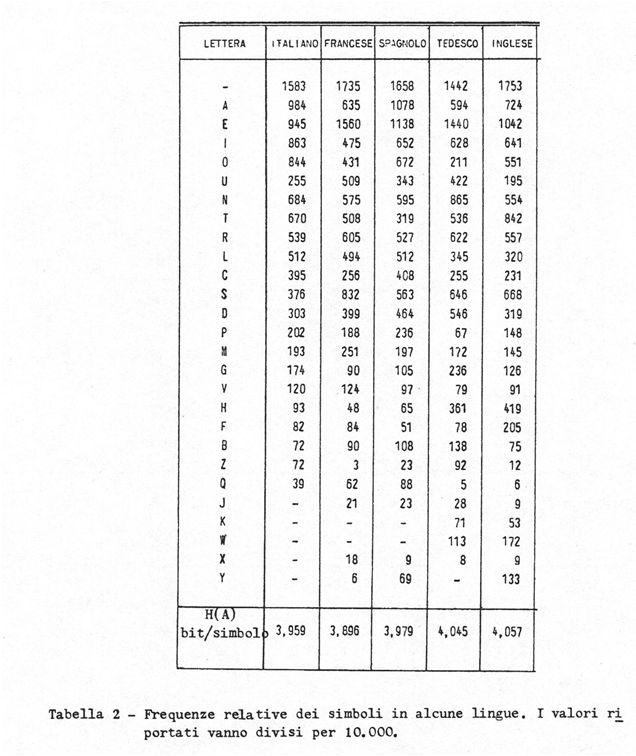
\includegraphics[scale = 1]{Entropy rate delle lingue.png}
\end{figure} 

dove, notiamo che, per la lingua inglese l'entropy rate H è uguale a: 

{
    \Large
    \begin{equation}
        H \approx 4.057 \frac{\text{bit}}{\text{simbolo}} 
    \end{equation}
}

L'entropy rate nel linguaggio parlato è molto più basso, perchè nel linguaggio c'è ridondanza. \newline 

Questo perchè, nel linguaggio parlato, si ripete più spesso la stessa parola, 
quindi, nell'insieme, la singola lettera porta una bassa informazione. \newline 

Grazie a queste considerazioni, avere una sorgente non d.m.s. con memoria può essere molto utile (anche se la trattazione matematica è più complessa), 
perchè può ottimizzare la trasmissione quando devo ridurre al minimo i simboli da inviare per trasmettere l'informazione (si pensi al caso del wifi dove la banda è limitata e ci sono tanti dispositivi connessi alla stessa rete contemporaneamente). \newline 

\newpage 

\section{Tributo a Claude Shannon}
\footnote{Slide del prof | Teoria dell'informazione | pag 8.2 \\  
Slide | Teoria dell'informazione | pag 8.2 \\
Appunti | 2025-03-21 | pag 3
}

\begin{tcolorbox}
    Grazie al socio Claude Shannon non potresti fare nulla al giorno d'oggi. \newline

    Il prof lo nomina almeno 3 miliardi di volte e fa bene. \newline 

    Senza Claude non riusciresti a vedere i video su Youtube, telefonare, inviare i video su Whatsapp e neanche ricevere la foto dei piedi di taglia 36 con smalto bianco della tipa che ti piace 
    (o la foto del tipo che ti piace in costume, qui non facciamo differenza di genere e gusti). \newline
    
    Ringrazia Claude Shannon per tutto questo. 
\end{tcolorbox}

\begin{figure}[h]
    \centering
    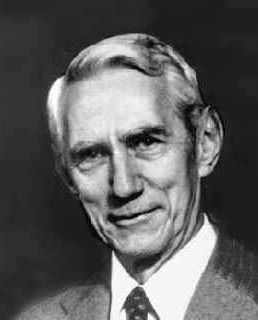
\includegraphics[scale = 1]{Claude Shannon.png}
\end{figure} 

Claude Shannon fu un matematico, pioniere della teoria matematica della comunicazione. \newline 

Grazie al suo paper "A Mathmatical Theory of Communication": 

\begin{figure}[h]
    \centering
    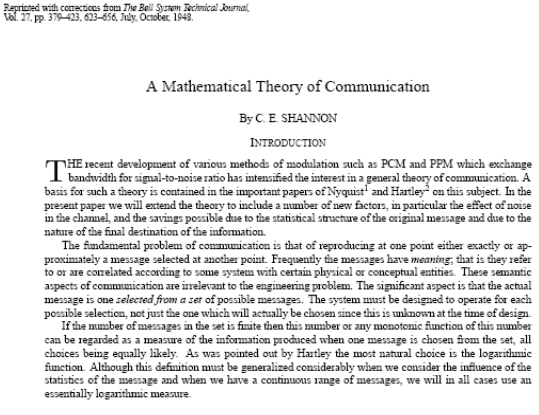
\includegraphics[scale = 1]{A Mathmatical Theory of Communication.png}
\end{figure} 

rivoluzionò le comunicazioni e permise di introdurre il concetto di codifica di sorgente. \newline 

\begin{tcolorbox}
    Se vuoi farti una bella lettura del paper "A Mathmatical Theory of Communication", ti lascio il link: \\
    \url{https://people.math.harvard.edu/~ctm/home/text/others/shannon/entropy/entropy.pdf}
\end{tcolorbox}

\newpage 

\subsection{Teorema della codifica di sorgente (Source Coding Theorem)}
\footnote{Slide del prof | Teoria dell'informazione | pag 9.1 \\  
Appunti di Damiano| pag 9.1 \\
Slide | Teoria dell'informazione | pag 9.1 \\
Appunti | 2025-03-21 | pag 4
}

Grazie al suo paper "A Mathmatical Theory of Communication", 
Claude Shannon introdusse diversi 23 teoremi, tra cui ne andremo ad analizzare uno: 
il teorema della codifica di sorgente, o in inglese Source Coding Theorem. \newline 

Di seguito il teorema: 

\begin{tcolorbox}[colback=yellow!5!white,colframe=black!75!black]
Una sorgente con entropia H(X) (o entropy rate H) può essere rappresentata, senza perdita di informazione, 
utilizzando un numero medio di simboli (ad esempio binari) per simbolo prodotto dalla sorgente che ha numero di simboli R:

{
    \Large 
    \begin{equation}
        R \ge H(X)
    \end{equation}
}

oppure: 

{
    \Large 
    \begin{equation}
        R \ge H
    \end{equation}
}

Se il numero dei simboli R è: 

{
    \Large 
    \begin{equation}
        R \le H(X)
    \end{equation}
}

oppure: 

{
    \Large 
    \begin{equation}
        R \le H
    \end{equation}
}

allora, l'informazione è sicuramente ridotta (quindi distorta), 
per quanto complesse siano le tecniche di rappresentazione utilizzate. 
\end{tcolorbox}

La rappresentazione dei simboli prodotti da una sorgente prende il nome di codifica di sorgente. \newline 

Shannon, grazie a questo teorema, impose il limite di codifica, cioè il limite sotto al quale non bisogna scendere per una trasmissione. \newline 

\newpage 

\subsection{Efficienza di codifica}
\footnote{Slide del prof | Teoria dell'informazione | pag 9.2 \\  
Appunti di Damiano| pag 9.2 \\
Slide | Teoria dell'informazione | pag 9.2 \\
Appunti | 2025-03-21 | pag 4
}

Come ribadito dal teorema della codifica, se: 

{
    \Large 
    \begin{equation}
        R \ge H(X)
    \end{equation}
}

cioè il numero di simboli R è maggiore dell'entropia H(X), non si ha perdita di informazione. \newline 

Si può definire il coefficiente di efficienza di codifica $\eta$: 

{
    \Large 
    \begin{equation}
        \eta 
        = 
        \frac{H (X)}{R}
    \end{equation}
}

dove:

\begin{itemize}
    \item se $\eta \le 1$ non si ha perdita di informazione perchè $R \ge H(X)$ 
    \item se $\eta > 1$ si ha perdita di informazione perchè $R < H(X)$ 
\end{itemize}

\newpage 

\subsubsection{Codifica di sorgente con sequenze codificate di lunghezza fissa}
\footnote{Slide del prof | Teoria dell'informazione | pag 10.1 \\  
Appunti di Damiano| pag 10.1 \\
Slide | Teoria dell'informazione | pag 10.1 \\
Appunti | 2025-03-21 | pag 4
}

Consideriamo il seguente esempio numerico. \newline 

Consideriamo di avere la seguente codifica di simboli: 

{
    \Large 
    \begin{center}
        \begin{tabular}{|c c|}
            \hline
            \textbf{Simbolo} & \textbf{Codifica} \\
            \hline 
            \hline
            $a_1$ & 000 \\
            $a_2$ & 001 \\
            $a_3$ & 010 \\
            $a_4$ & 011 \\
            $a_5$ & 100 \\
            \hline
        \end{tabular}
    \end{center}
}

Consideriamo la seguente tabella: 

\begin{figure}[h]
    \centering
    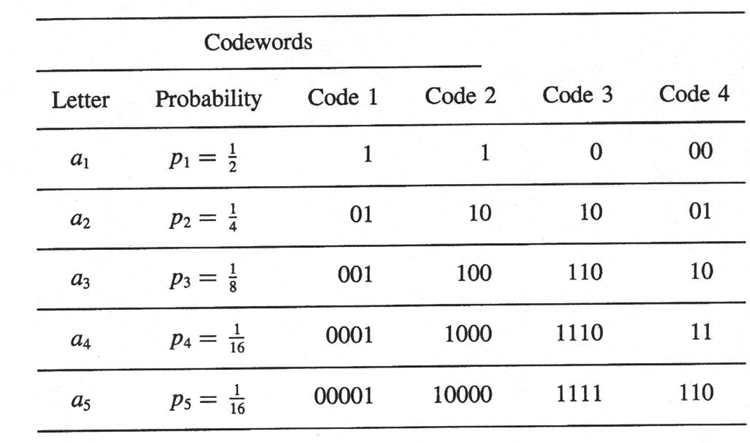
\includegraphics[scale = 1]{Tabella con codici a lunghrzza variabile.png}
\end{figure} 

Calcoliamoci l'entropia H(X) in cui il codice di codifica ha lunghezza fissa: 

{
    \Large
    \begin{equation}
        \begin{split}
            H (X)
            &= 
            \sum_{i = 1}^{N}
            p_i \cdot \log_{2} \left( \frac{1}{p_i}\right) 
            \\
            &= 
            \sum_{i = 1}^{5}
            p_i \cdot \log_{2} \left( \frac{1}{p_i}\right) 
            \\
            &= 
            \frac{1}{2} \cdot \log_2 (2) 
            +
            \frac{1}{4} \cdot \log_2 (4) 
            +
            \frac{1}{8} \cdot \log_2 (8) 
            +
            \frac{1}{16} \cdot \log_2 (16) 
            +
            \frac{1}{16} \cdot \log_2 (16)
            \\
            &= 
            \frac{1}{2} \cdot \log_2 (2) 
            +
            \frac{1}{4} \cdot \log_2 (4) 
            +
            \frac{1}{8} \cdot \log_2 (8) 
            +
            2 \cdot 
            \left(
            \frac{1}{16} \cdot \log_2 (16)
            \right)
            \\
            &=
            \frac{15}{8}
        \end{split}
    \end{equation}
}

\newpage 

\subsection{Sequenza di lunghezza variabile}
\footnote{Slide del prof | Teoria dell'informazione | pag 10.2 - 12.1 \\  
Appunti di Damiano| pag 10.2 - 12.1 \\
Slide | Teoria dell'informazione | pag 10.2 - 12.1 \\
Appunti | 2025-03-21 | pag 5 - 6
}

Se abbiamo lunghezze variabili, come facciamo a capire l'inizio e la fine di un simbolo? \newline 

Come si separano le parole di codice prodotte? \newline 

Tutte queste problematiche vengono risolte dall'auto-sincronizzazione. \newline 

Per applicare l'auto-sincronizzazione, bisogna applicare questo vincolo: 
non bisogna introdurre simboli ai fini della rappresentazione. \newline 

Ad esempio, nel caso binario dove abbiamo un alfabeto composto da 0 o 1, se usiamo il bit 1 per l'informazione, il bit 0 sarà quello che permetterà di dividere il simbolo da un altro. \newline 

Ma siccome non avremo mai a che fare con una lunghezza di due bit per rappresentare l'i-esimo simbolo, 
possiamo definire R numero di simboli come: 

{
    \Large 
    \begin{equation}
        R = \sum_{i = 1}^{N} L_i \cdot p_i
    \end{equation}
}

dove: 

\begin{itemize}
    \item $L_i$ è la lunghezza della rappresentazione dell'i-esimo simbolo 
    \item $p_i$ è la probabilità dell'i-esimo simbolo
\end{itemize}

Utilizzare una codifica in cui la lunghezza del simbolo è variabile porta un enorme vantaggio per la banda occupata, 
perchè la banda va calcolata in base a quanti bit si inviano nel canale. \newline 

Più bit bisogna inviare, più banda sarà richiesta nel canale. \newline 

Continuando l'esempio della sezione precedente, 
consideriamo la seguente tabella: 

\begin{figure}[h]
    \centering
    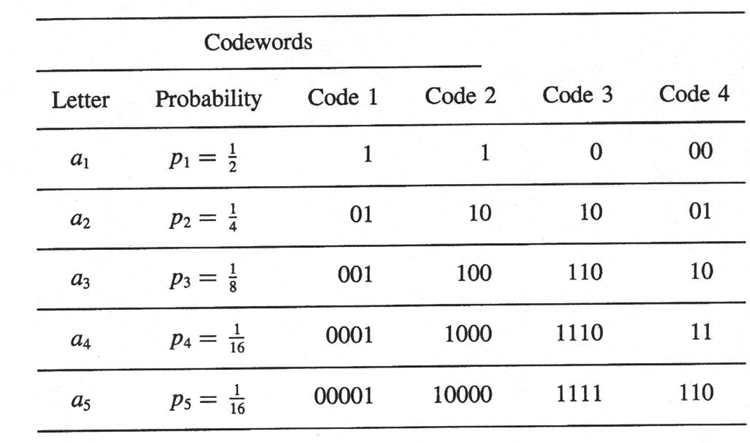
\includegraphics[scale = 1]{Tabella con codici a lunghrzza variabile.png}
\end{figure} 

Se consideriamo la colonna del primo codice (Code 1) abbiamo che N = 5 e che il numero dei simboli con questo codice $R_1$ vale: 

{
    \Large 
    \begin{equation}
        \begin{split}
            R_1
            &= 
            \sum_{i = 1}^{N}
            L_i \cdot p_i 
            \\
            &= 
            \sum_{i = 1}^{5}
            L_i \cdot p_i
            \\
            &= 
            L_1 \cdot p_1
            +
            L_2 \cdot p_2
            +
            L_3 \cdot p_3 
            + 
            L_4 \cdot p_4 
            + 
            L_5 \cdot p_5
            \\
            &= 
            1 \cdot \frac{1}{2}
            +
            2 \cdot \frac{1}{4}
            +
            3 \cdot \frac{1}{8} 
            + 
            4 \cdot \frac{1}{16} 
            + 
            5 \cdot \frac{1}{16}
            \\
            &= 
            \frac{31}{16}
        \end{split}
    \end{equation}
}

Se consideriamo l'entropia H(X) calcolata precedentemente con parola di codice di lunghezza fissa: 

{
    \Large 
    \begin{equation}
        H (X) = \frac{15}{8}
    \end{equation}
}

$R_1 \ge H(X)$, quindi con il codice 1 non si ha perdita di informazione. \newline 

Inoltre, il codice 1 è auto-sincronizzante perchè ogni parola di codice termina con un 1. \newline 

Ora facciamo gli stessi calcoli per il codice 2:

{
    \Large 
    \begin{equation}
        \begin{split}
            R_2
            &= 
            \sum_{i = 1}^{N}
            L_i \cdot p_i 
            \\
            &= 
            \sum_{i = 1}^{5}
            L_i \cdot p_i
            \\
            &= 
            L_1 \cdot p_1
            +
            L_2 \cdot p_2
            +
            L_3 \cdot p_3 
            + 
            L_4 \cdot p_4 
            + 
            L_5 \cdot p_5
            \\
            &= 
            1 \cdot \frac{1}{2}
            +
            2 \cdot \frac{1}{4}
            +
            3 \cdot \frac{1}{8} 
            + 
            4 \cdot \frac{1}{16} 
            + 
            5 \cdot \frac{1}{16}
            \\
            &= 
            \frac{31}{16}
        \end{split}
    \end{equation}
}

In questo caso, rispetto al codice 1, ogni parola di codice inizia con un 1, quindi è un codice auto-sincronizzante. \newline 

Contrariamente al codice 1, il codice 2 non è istantaneo perchè si deve attendere il primo simbolo della parola successiva per decidere che una parola di codice è terminata. \newline 

Invece, considerando il codice 3: 

{
    \Large 
    \begin{equation}
        \begin{split}
            R_3
            &= 
            \sum_{i = 1}^{N}
            L_i \cdot p_i 
            \\
            &= 
            \sum_{i = 1}^{5}
            L_i \cdot p_i
            \\
            &= 
            L_1 \cdot p_1
            +
            L_2 \cdot p_2
            +
            L_3 \cdot p_3 
            + 
            L_4 \cdot p_4 
            + 
            L_5 \cdot p_5
            \\
            &= 
            1 \cdot \frac{1}{2}
            +
            2 \cdot \frac{1}{4}
            +
            3 \cdot \frac{1}{8} 
            + 
            4 \cdot \frac{1}{16} 
            + 
            4 \cdot \frac{1}{16}
            \\
            &=
            1 \cdot \frac{1}{2}
            +
            2 \cdot \frac{1}{4}
            +
            3 \cdot \frac{1}{8} 
            + 
            2 \cdot
            \left(
                4 \cdot \frac{1}{16}
            \right)
            \\
            &= 
            \frac{30}{16}
            \\
            &= 
            \frac{15}{8}
        \end{split}
    \end{equation}
}

$R_3 = H (X)$, perchè non si ha perdita di informazione se $R_n \ge H(X)$ e quindi si considera anche la condizione di uguaglianza tra $R_n$ e H(X). \newline 

Ma, il problema del codice 3 è quello dell'auto-sincronizzazione perchè nessuna parola di codice è prefisso di un'altra parola di codice. \newline 

Invece, considerando il codice 4: 


{
    \Large 
    \begin{equation}
        \begin{split}
            R_4
            &= 
            \sum_{i = 1}^{N}
            L_i \cdot p_i 
            \\
            &= 
            \sum_{i = 1}^{5}
            L_i \cdot p_i
            \\
            &= 
            L_1 \cdot p_1
            +
            L_2 \cdot p_2
            +
            L_3 \cdot p_3 
            + 
            L_4 \cdot p_4 
            + 
            L_5 \cdot p_5
            \\
            &= 
            2 \cdot \frac{1}{2}
            +
            2 \cdot \frac{1}{4}
            +
            2 \cdot \frac{1}{8} 
            + 
            2 \cdot \frac{1}{16} 
            + 
            3 \cdot \frac{1}{16}
            \\
            &= 
            \frac{33}{16}
        \end{split}
    \end{equation}
}

$R_4 \ge H(X)$, quindi $R_4$ è informativo, ma pone il problema dell'auto-sincronizzazione. \newline 

Consideriamo la sequenza 110110. \newline 

Questa sequenza, con il codice 4, può provenire sia da $a_5 a_5$ che da $a_4 a_2 a_3$. \newline 

\newpage 

\subsection{Proprietà del prefisso (prefix condition)}
\footnote{Slide del prof | Teoria dell'informazione | pag 12.2 \\  
Appunti di Damiano| pag 12.2 \\
Slide | Teoria dell'informazione | pag 12.2 \\
Appunti | 2025-03-21 | pag 6
}

La proprietà del prefisso è una condizione necessaria e sufficiente affinché un codice (di sorgente) sia istantaneo ed univocamente decodificabile
(cioè auto-sincronizzante). \newline 

Per applicare questa proprietà, nessuna parola di codice è prefisso di un'altra parola di codice. \newline 

\newpage 

\subsection{Algoritmo di Huffman}
\footnote{Slide del prof | Teoria dell'informazione | pag 14.1 \\  
Appunti di Damiano| pag 14.1 \\
Slide | Teoria dell'informazione | pag 14.1 \\
Appunti | 2025-03-21 | pag 7
}

Considerando l'esempio precedente: 

\begin{figure}[h]
    \centering
    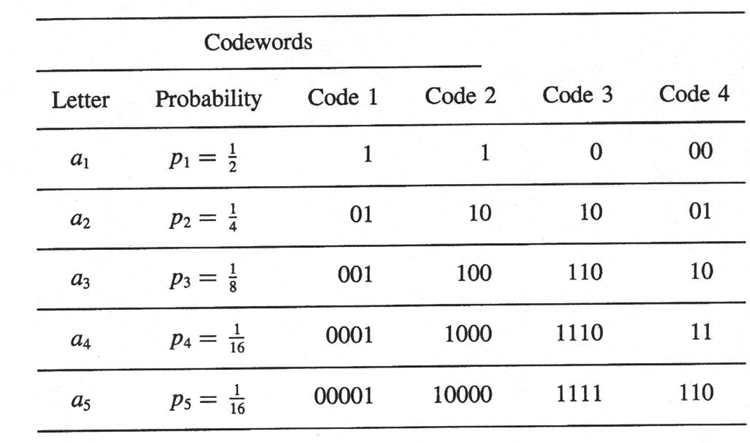
\includegraphics[scale = 0.6]{Tabella con codici a lunghrzza variabile.png}
\end{figure} 

il codice 3 implementa l'algoritmo di Huffman. \newline 

L'algoritmo di Huffman trasforma le sequenze di lunghezza fissa in sequenze di codice di lunghezza variabile. \newline 

L'idea è quella di rappresentare i simboli (o le sequenze) di informazione più probabili con le parole di codice più corte. \newline 

Per essere applicato, bisogna avere un codice ottimo in cui si ha questa relazione: 

{
    \Large
    \begin{equation}
        H (X) \le R \le H(X) + 1
    \end{equation}
}

Se $p_i$: 

{
    \Large 
    \begin{equation}
        p_i = \frac{1}{2^{k}}
    \end{equation}
}

dove k sono i bit, allora il codice si dice perfettamente ottimo perchè vale questa relazione: 

{
    \Large 
    \begin{equation}
        R = H(X)
    \end{equation}
}

Ritornando all'esempio in figura, il codice 3 è perfettamente ottimo. \newline 

L'algoritmo di Huffman viene utilizzato negli standard JPEG e MPEG per la codifica video. \newline 

\newpage 

\subsubsection{Algoritmo di Huffman: implementazione scalare e binaria}
\footnote{Slide del prof | Teoria dell'informazione | pag 14.2 - 15 \\  
Appunti di Damiano| pag 14.2 - 15 \\
Slide | Teoria dell'informazione | pag 14.2 - 15 \\
Appunti | 2025-03-24 | pag 2 - 3
}

L'algoritmo di Huffman, utilizzando lo schema a blocchi, è il seguente: 

\begin{figure}[h]
    \centering
    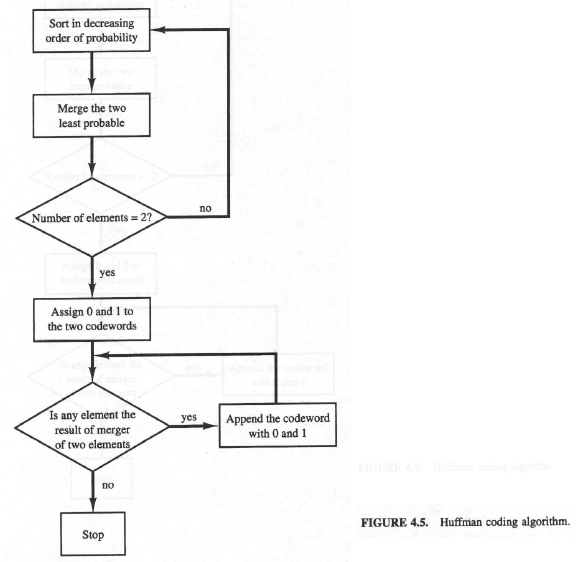
\includegraphics[scale = 1]{Algortitmo di Huffman schema a blocchi.PNG}
\end{figure} 

Dal punto di vista testuale, step-by-step, 
l'algoritmo di Huffman si implementa in questa maniera seguendo questi passaggi: 

\begin{enumerate}
    \item Si ordinano le probabilità $p_i$ in modo decrescente (quindi dalla probabilità più alta a quella meno probabile)
    \item Si uniscono i due simboli in ingresso meno probabili in un unico simbolo, la cui probabilità è la somma delle probabilità corrispondenti 
    \item Se il numero dei simboli si è ridotto a 2, si passa al punto successivo, altrimenti si ritorna al punti 1 
    \item Si assegnano (arbitrariamente) 0 e 1 ai due simboli rimanenti (da ciò deriva il famoso logaritmo in base 2) 
    \item Si percorrono le operazioni fatte in precedenza: ogni volta che si erano uniti due simboli, si associa 0 a uno dei due simboli e 1 all'altro 
    \item Le parole di codice risultano dalla concatenazione degli 0 e degli 1 così assegnati
\end{enumerate}

\newpage 

Ritornando all'esempio della tabella in cui si confrontano i codici: 

\begin{figure}[h]
    \centering
    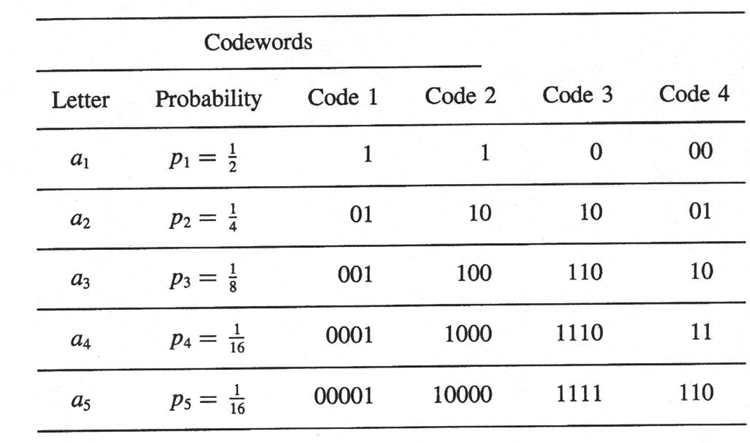
\includegraphics[scale = 0.6]{Tabella con codici a lunghrzza variabile.png}
\end{figure} 

considerando il codice 3 in cui è stato implementato l'algoritmo di Huffman, 
possiamo visualizzare l'albero e le probabilità con lo schema seguente: 

\begin{figure}[h]
    \centering
    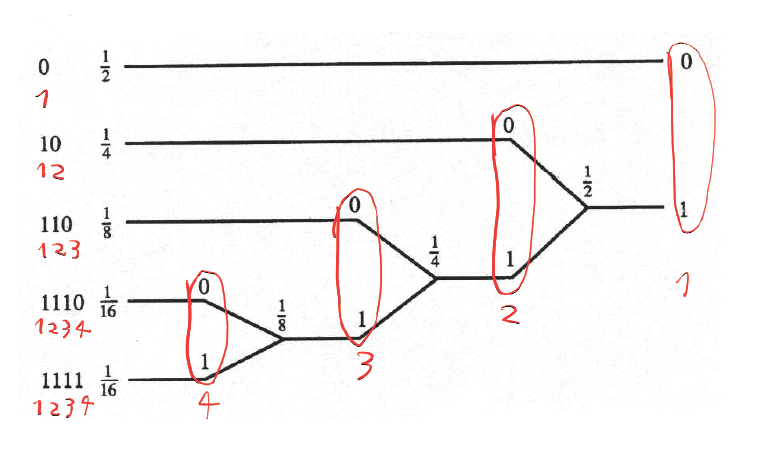
\includegraphics[scale = 0.6]{Algortitmo di Huffman applicazione.PNG}
\end{figure} 

(dove, nella figura, sono segnati i percorsi che il numero ha svolto per far corrispondere a quella probabilità). \newline 

\newpage 

\subsubsection{Algoritmo di Huffman: implementazione vettoriale}
\footnote{Slide del prof | Teoria dell'informazione | pag 16 - 18.1\\  
Appunti di Damiano| pag 16 - 18.1 \\
Slide | Teoria dell'informazione | pag 16 - 18.1 \\
Appunti | 2025-03-24 | pag 3 - 4
}

Si può implementare l'algoritmo di Huffman codificando n simboli alla volta. \newline 

In questo caso, R deve essere: 

{
    \Large
    \begin{equation}
        H(X) \le R \le H(X) + \frac{1}{n}
    \end{equation}
}

dove n sono i simboli codificati simultaneamente. \newline 

Possiamo considerare il limite in cui n tende a infinito. \newline 

In quel caso R deve essere: 

{
    \Large 
    \begin{equation}
        R = H(X) \text{ per } n \to + \infty
    \end{equation}
}

Consideriamo di avere la seguente codifica di simboli: 

{
    \Large 
    \begin{center}
        \begin{tabular}{|c c|}
            \hline
            \textbf{Simbolo} & \textbf{Codifica} \\
            \hline 
            \hline
            $a_1$ & 000 \\
            $a_2$ & 001 \\
            $a_3$ & 010 \\
            $a_4$ & 011 \\
            $a_5$ & 100 \\
            \hline
        \end{tabular}
    \end{center}
}

si possono implementare dei codici in cui si codificano due simboli alla volta, quindi n = 2. \newline 

\newpage 

Di seguito delle rappresentazioni dell'algoritmo di Huffman con questa codifica: 

\begin{figure}[h]
    \centering
    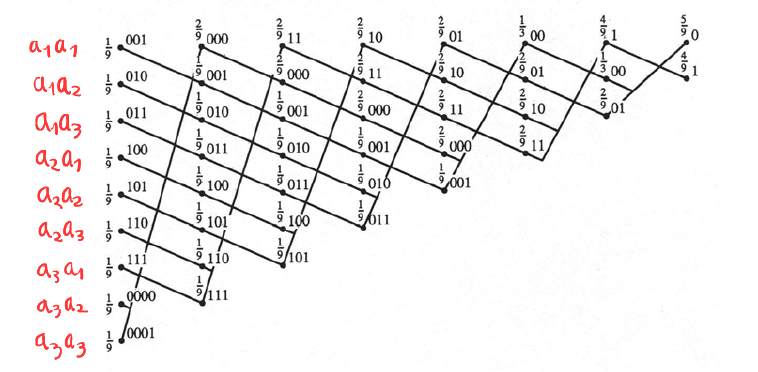
\includegraphics[scale = 1]{Algoritmo di Huffman implementazione vettoriale.PNG}
\end{figure} 

oppure: 

\begin{figure}[h]
    \centering
    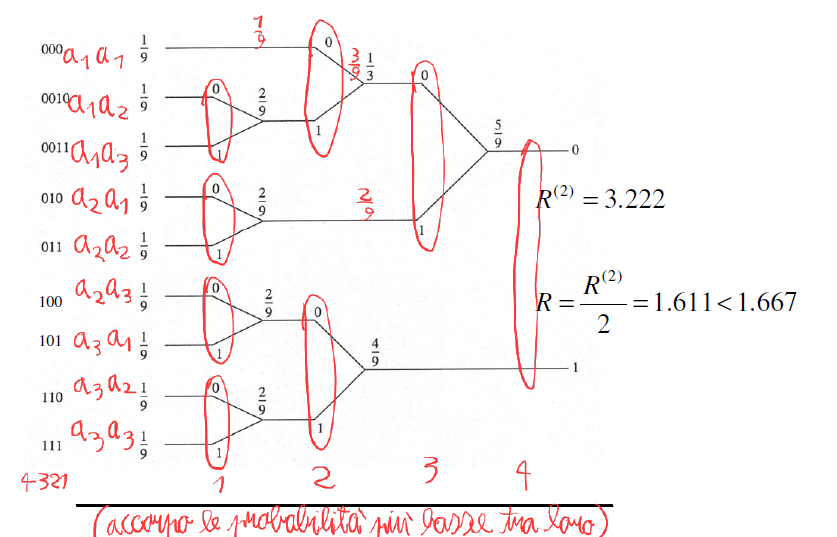
\includegraphics[scale = 1]{Algoritmo di Huffman implementazione vettoriale 2.PNG}
\end{figure} 

\newpage 

\subsection{Algoritmo di Lempel-Ziv}
\footnote{Slide del prof | Teoria dell'informazione | pag 18.2 \\  
Appunti di Damiano| pag 18.2 \\
Slide | Teoria dell'informazione | pag 18.2 \\
Appunti | 2025-03-24 | pag 5
}

L'algoritmo di Lempel-Ziv trasforma sequenze di informazione di lunghezza variabile in sequenze di codice di lunghezza fissa. \newline 

Implementando una lunghezza fissa, l'algoritmo di Lempel-Ziv non ha problemi di sincronizzazione come Huffman. \newline 

Questo tipo di algoritmo è "duale" al codice di Huffman e cerca di risolvere i problemi di Huffman che sono i seguenti: 

\begin{itemize}
    \item occorre conoscere la distribuzione di probabilità 
    \item l'implementazione vettoriale è complessa
\end{itemize}

Anche l'algoritmo di Lempel-Ziv è ottimo perchè le parole di codice verificano la proprietà del prefisso ed hanno lunghezza minima. \newline 

Si dice che l'algoritmo di Lempel-Ziv è un algoritmo di codifica di sorgente universale perchè non ha bisogno di conoscere la statistica della sorgente a priori. \newline 

Questo tipo di algoritmo è impiegato principalmente nella compressione dei file, ad esempio i file .zip .\newline 

\newpage 

\subsubsection{Algoritmo di Lempel-Ziv: esempio}
\footnote{Slide del prof | Teoria dell'informazione | pag 19 - 21.1\\  
Appunti di Damiano| pag 19 - 21.1\\
Slide | Teoria dell'informazione | pag 19 - 21.1 \\
Appunti | 2025-03-24 | pag 5 - 6
}

Si considera la sequenza: 

{
    \Large
    \begin{equation}
        0100001100001010000010100000110000010100001001001
    \end{equation}
}

Il primo step è implementare un parsing, cioè si suddivide la stringa in piccoli frasi. \newline 

Cioè: 

{
    \Large 
    \begin{equation}
        \begin{split}
           010000110000101000001010&0000110000010100001001001
           \\
           &\downarrow
           \\
           0, 1, 00, 001, 10, 000, 101, 0000, &01, 010, 00001, 100, 0001, 0100, 0010, 01001 
        \end{split}
    \end{equation}
}

Ogni frase è composta da una sequenza di 0 e 1 "nuova", ovvero è diversa ogni frase individuata precedentemente. \newline 

Scorrendo la sequenza in ingresso, 
una nuova frase è data dalla sequenza di lunghezza minima non ancora trovata in precedenza. \newline 

Ad esempio, la terza frase 00 è data dalla prima frase che è 0 più 0, la frase 001 è data dalla terza frase che è 00 più 1 e così via. \newline 

Il secondo step è memorizzare le frasi in una memoria indicizzata, come nel seguente caso: 

\begin{figure}[h]
    \centering
    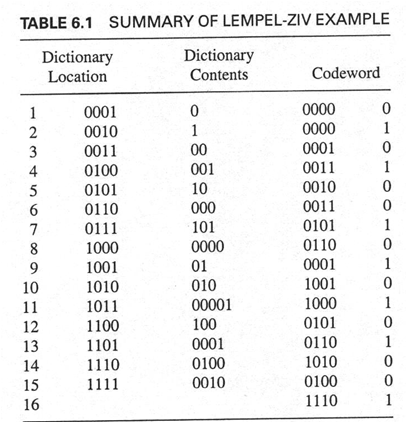
\includegraphics[scale = 1]{Memoria indicizzata con Lempel-Ziv.png}
\end{figure} 

Il terzo step è quello della codifica, in cui la parola di codice associata ad ogni frase è: 

\begin{itemize}
    \item la concatenazione dell'indirizzo della sequenza d'informazione da cui la frase deriva 
    \item la novità della frase
\end{itemize}

\begin{tcolorbox}
    Devo ammettere che così spiegato l'algoritmo di Lempel-Ziv è spiegato con i piedi. \newline 

    Ti lascio due video al riguardo. \newline 

    \url{https://youtu.be/RV5aUr8sZD0?si=Fkt7DbrBK-WrSzUK}\\
    Lossless Compression: Lempel-Ziv by Art of the Problem \newline 

    \url{https://www.youtube.com/watch?v=Jqc418tQDkg}\\
    Why the Lempel-Ziv algorithms are so dominant by Google for Developers
\end{tcolorbox}

Se la sequenza di bit è molto breve, con l'algoritmo di Lempel-Ziv non si ha una compressione (anzi, si allunga la sequenza), 
ma diventa efficace quando si ha una sequenza molto lunga perchè le frasi si ripetono e si fanno riferimento alla frasi precedenti, fino ad arrivare a 0 e 1. \newline 

La lunghezza della parola di codice è determinata dalla scelta fatta per la dimensione della memoria. \newline 

Il processo per cui si prende nella codifica alcune locazioni che sono più richiamate e possono essere riutilizzate prende il nome di purging. \newline 

L'efficienza dell'algoritmo dipende dal purging: più viene utilizzato, e più l'algoritmo è efficiente. \newline 


\newpage 

\section{Rate-distortion theory}
\footnote{Slide del prof | Teoria dell'informazione | pag 21.2 \\  
Appunti di Damiano| pag 21.2 \\
Slide | Teoria dell'informazione | pag 21.2 \\
Appunti | 2025-03-24 | pag 6 - 7
}

Da Shannon, sappiamo che se: 

{
    \Large 
    \begin{equation}
        R < H(X)
    \end{equation}
}

sicuramente l'informazione sarà distorta. \newline 

Ma, nonostante ciò, possiamo minimizzarla: in alcuni casi non abbiamo memoria per avere R abbastanza grande (si pensi alla memoria di un microcontrollore). \newline 

Quindi, l'obbiettivo per minimizzare la perdita di informazione è scegliere uno dei due apporci:

\begin{itemize}
    \item per un dato R, minimizzare la distorsione D 
    \item per una data distorsione D, minimizzare R
\end{itemize}

\begin{tcolorbox}
    Come dice il detto: non puoi avere insieme la botte piena e la moglie ubriaca. \newline 

    Bisogna trovare un compromesso, e molte delle volte è scegliere quanto perdere
\end{tcolorbox}

\newpage 

\subsection{Misura della distorsione}
\footnote{Slide del prof | Teoria dell'informazione | pag 22.1 \\  
Appunti di Damiano| pag 22.1 \\
Slide | Teoria dell'informazione | pag 22.1 \\
Appunti | 2025-03-24 | pag 7
}

Consideriamo x(t) il segnale "originale" e $\hat{x}$(t) la rappresentazione di x(t). \newline 

Si possono dare innumerevoli definizioni di distorsione D. \newline 

Di seguito alcune definizioni di D: 

{
    \Large 
    \begin{equation}
        D = \max_t \abs{x (t) - \hat{x} (t)}
    \end{equation}
}

{
    \Large 
    \begin{equation}
        D = \lim_{T \to \infty} \frac{1}{T} \int_{- \frac{T}{2}}^{+ \frac{T}{2}} \abs{x (t) - \hat{x} (t)} dt
    \end{equation}
}


{
    \Large 
    \begin{equation}
        D = \lim_{T \to \infty} \frac{1}{T} \int_{- \frac{T}{2}}^{+ \frac{T}{2}} \left[x (t) - \hat{x} (t) \right]^{2} dt
    \end{equation}
}

La distorsione D deve corrispondere alle proprietà "sensibili" in fase di rivelazione, e deve essere semplice da calcolare. \newline 

\newpage 

\subsubsection{Distanza di Hamming}
\footnote{Slide del prof | Teoria dell'informazione | pag 22.2 \\  
Appunti di Damiano| pag 22.2 \\
Slide | Teoria dell'informazione | pag 22.2 \\
Appunti | 2025-03-24 | pag 7
}

La distorsione è una misura della distanza tra x e la sua rappresentazione $\hat{x}$. \newline 

Definiamo distanza di Hamming $d_H$ tra x e $\hat{x}$ se:

{
    \Large 
    \begin{equation}
        d_H (x, \hat{x})
        = 
        \begin{cases}
            1 \text{ se } x \neq \hat{x}
            \\
            0 \text{ se } x = \hat{x}
        \end{cases}
    \end{equation}
}

Questo tipo distanza di Hamming viene definita come distanza hard perchè può assumere solo due valori. \newline 


\begin{tcolorbox}
    La distanza di Hamming può avere più definizioni. \newline 
    
    In questo corso vediamo questa qui, cioè la distanza di Hamming applicata al calcolo probabilistico. \newline  

    Se vuoi farti una cultura sul perchè Hamming fu rivoluzionario, guardati questo video: \newline 

    \url{https://www.youtube.com/watch?v=X8jsijhllIA&t=171s} \\
    But what are Hamming codes? The origin of error correction by 3Blue1Brown
\end{tcolorbox}

\newpage 

\subsubsection{Distanza in media quadratica}
\footnote{Slide del prof | Teoria dell'informazione | pag 23.1 \\ 
Appunti di Damiano| pag 23.1 \\
Slide | Teoria dell'informazione | pag 23.1 \\
Appunti | 2025-03-24 | pag 7
}

Possiamo definire una distanza d in media quadratica tra x e la sua rappresentazione $\hat{x}$ come: 

{
    \Large 
    \begin{equation}
        d (x, \hat{x}) = (x - \hat{x})^{2}
    \end{equation}
}

In questo caso, $d (x, \hat{x}) $ viene definita come distanza soft, perchè, a differenza della distanza hard dove assume solo due valori, 
questa distanza assume diversi valori, che, grazie alla definizione, tende a zero se la differenza tra x $\hat{x}$ è quasi nulla, 
la distanza aumenta se x e $\hat{x}$ diventano sempre più diversi. \newline 

\newpage 

\subsubsection{Distanza tra vettori}
\footnote{Slide del prof | Teoria dell'informazione | pag 23.2 \\  
Appunti di Damiano| pag 23.2 \\
Slide | Teoria dell'informazione | pag 23.2 \\
Appunti | 2025-03-24 | pag 8
}

Definiamo $\mathbf{x}^{n}$ un vettore composto da n elementi e $\hat{\mathbf{x}}^{n}$ la rappresentazione di $\mathbf{x}^{n}$. \newline 

Possiamo definire la distanza d tra $\mathbf{x}^{n}$ e $\hat{\mathbf{x}}^{n}$ come: 

{
    \Large 
    \begin{equation}
        d(\mathbf{x}^{n}, \hat{\mathbf{x}}^{n}) = \frac{1}{n} \cdot \sum_{i = 1}^{n} d(x_i, \hat{x_i})
    \end{equation}
}

dove $x_i$ e $\hat{x_i}$ è il singolo elemento del vettore, rispettivamente, di $\mathbf{x}^{n}$ e $\hat{\mathbf{x}}^{n}$. \newline 

\begin{tcolorbox}
    Se non ti ricordi come è e cosa è un vettore, in informatica, si intendono questi: 

    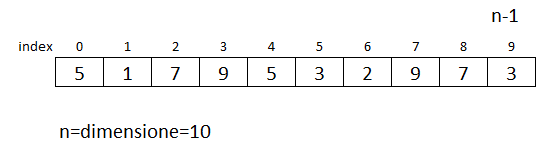
\includegraphics[scale = 1]{struttura-vettore.png}
\end{tcolorbox}

Nel caso probabilistico, possiamo definire la distanza D tra i vettori $\mathbf{X}^{n}$ e $\hat{\mathbf{X}}^{n}$ . \newline 

{
    \Large 
    \begin{equation}
        \begin{split}
            D 
            &= 
            \mathbb{E} \left[ d(\mathbf{X}^{n}, \hat{\mathbf{X}}^{n}) \right] 
            \\
            &= 
            \frac{1}{n}
            \cdot 
            \sum_{i = 1}^{n}
            \mathbb{E} \left[ d(X_i, \hat{X_i}) \right]_{\text{stazionarietà}}
            \\
            &= 
            \mathbb{E} \left[ d(X, \hat{X}) \right]
        \end{split}
    \end{equation}
}

dove con la lettera $\mathbb{E}$ si intende la media dei valori degli argomenti. \newline 

In questo caso, $\mathbb{E} \left[ d(\mathbf{X}^{n}, \hat{\mathbf{X}}^{n}) \right] $ si intende la media delle distanza tra i vettori $\mathbf{X}^{n}$ e $\hat{\mathbf{X}}^{n}$. \newline 

\newpage 

\subsubsection{Distanza nel caso di distanza $d_H$}
\footnote{Slide del prof | Teoria dell'informazione | pag 24.1 \\  
Appunti di Damiano| pag 24.1 \\
Slide | Teoria dell'informazione | pag 24.1 \\
Appunti | 2025-03-24 | pag 8
}

Nel caso di utilizzare la definizione di distanza di Hamming $d_H$: 

{
    \Large 
    \begin{equation}
        d_H (x, \hat{x})
        = 
        \begin{cases}
            1 \text{ se } x \neq \hat{x}
            \\
            0 \text{ se } x = \hat{x}
        \end{cases}
    \end{equation}
}

possiamo definire la distanza D tra X e $\hat{X}$ come: 

{
    \Large 
    \begin{equation}
        \begin{split}
            D 
            &=
            \mathbb{E} \left[ d(X, \hat{X}) \right]
            \\
            &\downarrow
            \\
            D 
            &=
            \mathbb{E} \left[ d_H(X, \hat{X}) \right]
            \\
            &= 
            1 \cdot \Pr{X \neq \hat{X}}
            +
            0 \cdot \Pr{X \neq \hat{X}}
            \\
            &=
            \Pr{X \neq \hat{X}} + 0 
            \\
            &= 
            \Pr{X \neq \hat{X}}
            \\
            &= 
            \Pr{\text{errore}}
        \end{split}
    \end{equation}
}

Da questa dimostrazione, quando si utilizza la distanza di Hamming, la distorsione D coincide con la probabilità di errore $\Pr{\text{errore}}$. \newline 


\newpage 
